\documentclass[11pt,a4paper]{article}
\usepackage[utf8]{inputenc}
\usepackage[spanish]{babel}
\usepackage{amsmath}
\usepackage{amsfonts}
\usepackage{amssymb}
\usepackage{graphicx}
\usepackage[left=2cm,right=2cm,top=2cm,bottom=2cm]{geometry}
\title{Universidad Politécnica de la Zona Metropolitana de Guadalajara}
\begin{document}

\maketitle
\begin{figure}[h]
\begin{center}

\includegraphics[scale=1]{1.jpeg}
\end{center}
\end{figure}

\begin{center}
\author{Sistemas Electrónicos de Interfaz\\
Barrera Vazquez Omar\\
Ing. Mecatrónica 4B}
\end{center}

\newpage

\section{Objetivo general}

Aplicar e integrar los conocimientos obtenidos sobre las tareas de \emph{tiristores} en reguladores de corriente y voltaje, los cuales son aplicados en un \emph{Dimmer} regulador de la intensidad lumínica de una bombilla incandescente en cual también se aplican conocimientos básicos de capacitores y resistencias en AC (corriente alterna).

\section{Materiales}

Los materiales a utilizar en esta practica son básicos, de bajo costo y fácil de conseguir, son los siguientes:

\begin{itemize}

\item 1 resistencia de 1k$\Omega$
\item 1 resistencia variable de 500k$\Omega$
\item 1 tiristor tipo DIAC
\item 1 tiristor tipo TRIAC
\item 1 clavija para corriente alterna 127V
\item 1 capacitor cerámico de 1$\mu$faradio
\item 1 Protoboard
\item cable para protoboard 

\end{itemize}

\section{Diagrama en funcionamiento}

El diagrama compuesto por los materiales mencionados en la sección \emph{2.materiales} se muestran en un diagrama que hará la regulación del voltaje como lo muestra la figura 1:

\begin{figure}[h]
\begin{center}
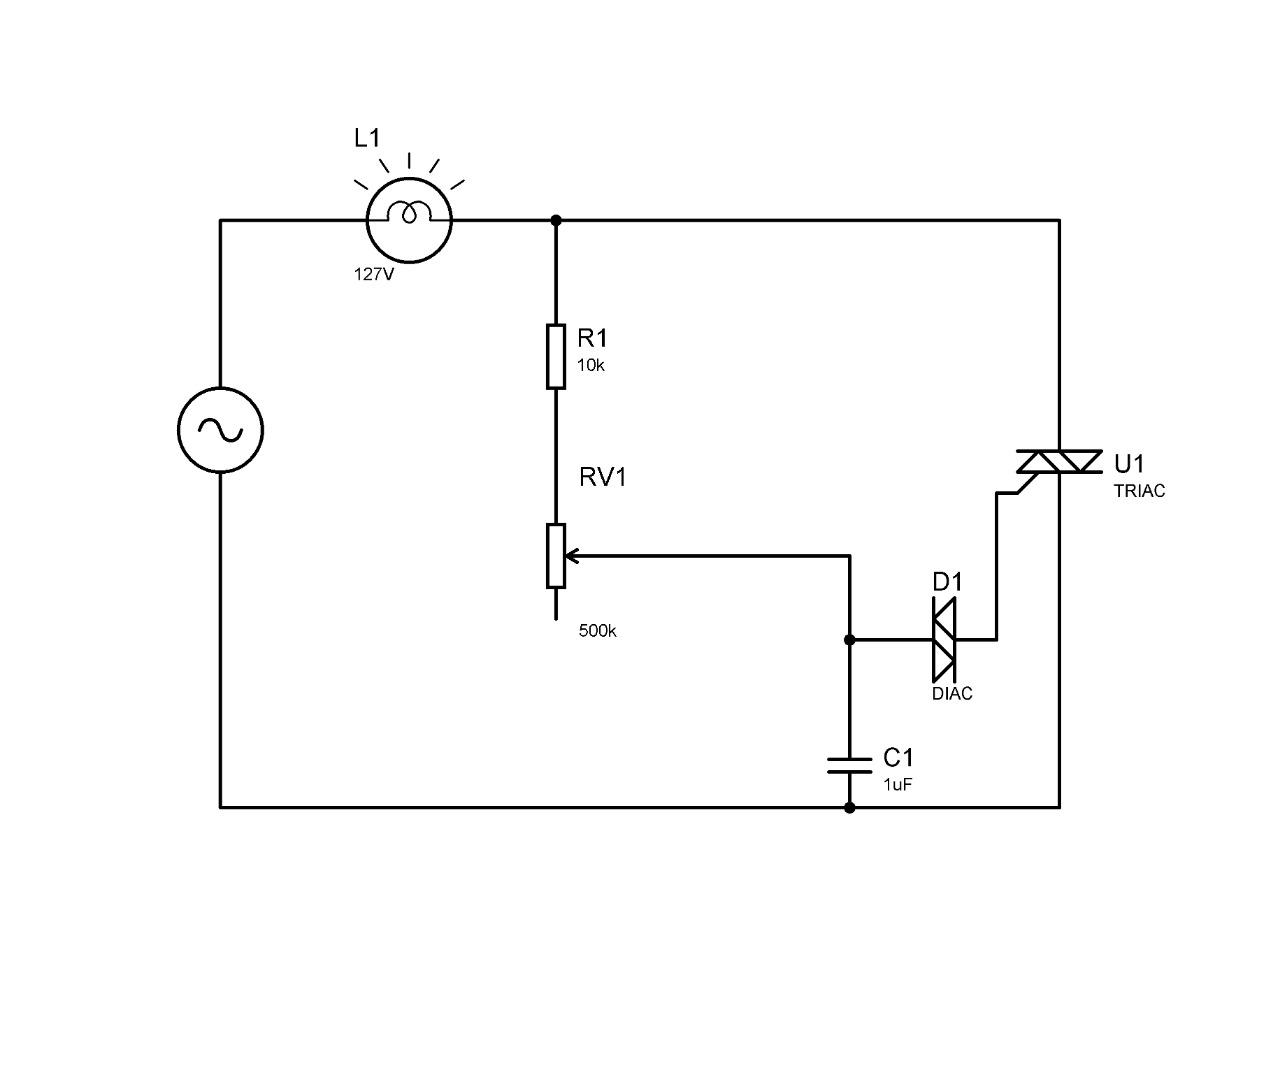
\includegraphics[scale=0.2]{2.jpeg}
\caption{diagrama eléctrico de Dimmer}
\end{center}
\end{figure}

\newpage

\textbf{Resistencia variable} como se observa en el diagrama eléctrico, quien controlara la intensidad de la luminosidad de la lampara incandescente sera la resistencia variable la cual al ir disminuyendo su capacidad resistiva no dará un mayor paso de la corriente.\\

\begin{figure}[h]
\begin{center}
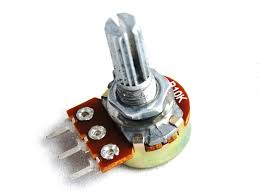
\includegraphics[scale=0.4]{3.jpeg}
\caption{resistencia variable o potenciómetro}
\end{center}
\end{figure}


\textbf{resistencia 1k$\Omega$} la resistencia de 1k$\Omega$ nos servirá como una resistencia de protección en caso de que la resistencia variable quede en 0$\Omega$ por lo cual nos dejara una carga resistiva.\\

\begin{figure}[h]
\begin{center}
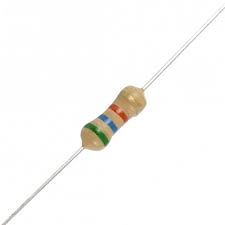
\includegraphics[scale=0.4]{4.jpeg}
\caption{resistencia de carbón}
\end{center}
\end{figure}


\textbf{Capacitor} el capacitor nos dará la función de almacenar un voltaje que soltara una vez  alcance los 30V que necesita el DIAC, es importante mencionar que el capacitor tiene que ser cerámico.\\

\begin{figure}[h]
\begin{center}
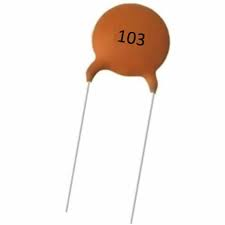
\includegraphics[scale=0.4]{5.jpeg}
\caption{capacitor tipo cerámico}
\end{center}
\end{figure}


\newpage

\textbf{DIAC} el DIAC es un tipo de tiristor bipolar semicontrolado, el cual este modelo en especifico hace una apertura de conducción cuando recibe 30V, lo que hace permitir el paso de la corriente a través de el.\\

\begin{figure}[hb]
\begin{center}
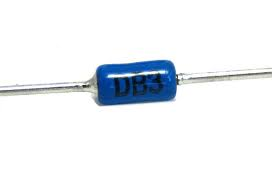
\includegraphics[scale=0.4]{6.jpeg}
\caption{tiristor tipo DIAC}
\end{center}
\end{figure}

\textbf{TRIAC} el TRIAC es un tiristor controlado por pulsos eléctricos que recibe en su \emph{GATE} el cual funciona de manera bipolar.\\

\begin{figure}[h]
\begin{center}
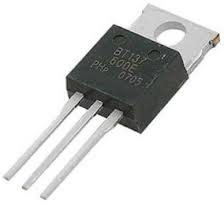
\includegraphics[scale=0.4]{7.jpeg}
\caption{tiristor tipo TRIAC}
\end{center}
\end{figure}

\section{Resultados}
Al momento que activamos el circuito en la practica obtendremos una variación de intensidad como la que se muestra la figura 7 en la cual dependerá de la variación de la resistencia variable:

\begin{center}

\begin{tabular}{|c|c|c|}
\hline 
\multicolumn{3}{|c|}{Nivel de intensidad según resistencia} \\ 
\hline 
1era fase & 500k$\Omega$ & foco apagado \\ 
\hline 
2da fase & 350k$\Omega$ & foco tenue \\ 
\hline 
3era fase & 141k$\Omega$ & foco luminoso 1 \\ 
\hline 
4ta fase & 0k$\Omega$ & foco luminoso 2 \\ 
\hline 
\end{tabular} 

\end{center}


\section{Conclusión}

La utilización para el control el paso de la corriente en circuitos AC (corriente alterna) es de gran utilidad por ser dispositivos semicontrolados y controlados por sistemas  de control como PLC o simples interruptores y vareadores de energía. El Dimmer es un dispositivo de claro ejemplo el cual es un variado de voltaje y corriente por medio de dispositivos controlados como lo son los TRIAC y DIAC.



\end{document}